\documentclass[a4paper, 12pt]{article}

\usepackage{graphicx}
\usepackage{float}
\graphicspath{ {img/} }

\newcommand{\templates}{../../template}
\usepackage[a4paper, margin=2.5cm]{geometry}

\usepackage{enumitem}
\setlist[itemize]{noitemsep}
\setlist[enumerate]{noitemsep}

\let\oldpar\paragraph
\renewcommand{\paragraph}[1]{\oldpar{#1\\}\noindent}

% Avoid dots in the table of contents, it mess with the gulpease calculation
\makeatletter
\renewcommand{\@dotsep}{10000} 
\makeatother
\usepackage{graphicx}
\usepackage{hyperref}
\usepackage{makecell}
\usepackage{fancyhdr}

\newcommand{\settitolo}[1]{\newcommand{\titolo}{#1\\}}
\newcommand{\setprogetto}[1]{\newcommand{\progetto}{#1\\}}
\newcommand{\setcommittenti}[1]{\newcommand{\committenti}{#1\\}}
\newcommand{\setredattori}[1]{\newcommand{\redattori}{#1\\}}
\newcommand{\setrevisori}[1]{\newcommand{\revisori}{#1\\}}
\newcommand{\setresponsabili}[1]{\newcommand{\responsabili}{#1\\}}
\newcommand{\setversione}[1]{
	\ifdefined\versione\renewcommand{\versione}{#1\\}
	\else\newcommand{\versione}{#1\\}\fi
}
\newcommand{\setdestuso}[1]{\newcommand{\uso}{#1\\}}
\newcommand{\setdescrizione}[1]{\newcommand{\descrizione}{#1\\}}

\newcommand{\makefrontpage}{
	\begin{titlepage}
		\begin{center}

		
\includegraphics[width=0.4\textwidth]{\templates/4ourSquared_logo}\\

		{\Large 4OURSQUARED}\\[6pt]
		\href{mailto://4oursquared.unipd@gmail.com}{4oursquared.unipd@gmail.com}\\
		
		\ifdefined\progetto
		\vspace{1cm}
		{\Large\progetto}
		{\large\committenti}
		\else\fi
		
		\vspace{1.5cm}
		{\LARGE\titolo}
		
		\vfill
		
		\begin{tabular}{r | l}
		\multicolumn{2}{c}{\textit{Informazioni}}\\
		\hline
		
		\ifdefined\redattori
			\textit{Redattori} &
			\makecell[l]{\redattori}\\
		\else\fi
		\ifdefined\revisori
			\textit{Revisori} &
			\makecell[l]{\revisori}\\
		\else\fi
		\ifdefined\responsabili
			\textit{Responsabili} &
			\makecell[l]{\responsabili}\\
		\else\fi
		
		\ifdefined\versione
			\textit{Versione} & \versione
		\else\fi
		
		\textit{Uso} & \uso
		
		\end{tabular}
		
		\vspace{2cm}
		
		\ifdefined\descrizione
		Descrizione
		\vspace{6pt}
		\hrule
		\descrizione
		\else\fi
		\end{center}
	\end{titlepage}
}
\usepackage{hyperref}
\usepackage{array}
\usepackage{tabularx}
\usepackage{adjustbox}

\newcounter{verscount}
\setcounter{verscount}{0}
\newcommand{\addversione}[5]{
	\ifdefined\setversione
		\setversione{#1}
	\else\fi
	\stepcounter{verscount}
	\expandafter\newcommand%
		\csname ver\theverscount \endcsname{#1&#2&#3&#4&#5}
}

\newcommand{\listversioni}{
	\ifnum\value{verscount}>1
		\csname ver\theverscount \endcsname
		\addtocounter{verscount}{-1}
		\\\hline
		\listversioni
	\else
		\csname ver\theverscount \endcsname\\\hline
	\fi
}

\newcommand{\makeversioni}{
	\begin{center}
		\begin{tabularx}{\textwidth}{|c|c|c|c|X|}
		\hline
		\textbf{Versione} & \textbf{Data} & \textbf{Redattore} & \textbf{Verificatore} & \textbf{Descrizione} \\
		\hline
		\listversioni
		\end{tabularx}
	\end{center}
	\clearpage
}

\settitolo{Manuale Manutentore}
\setprogetto{Lumos Minima}
\setcommittenti{Imola Informatica}
\setredattori{Soldà Matteo}
\setdestuso{esterno}
\setdescrizione{
Questo documento descrive le funzionalità del programma a coloro che dovessero usufruirne in qualità di utente con privilegi di base.
}

\addversione{0.0.0}{05/09/2023}{Soldà Matteo}{}{Stesura scheletro}
\addversione{0.0.1}{07/09/2023}{Soldà Matteo}{}{Stesura prima bozza contenuto}
\addversione{0.0.2}{13/09/2023}{Soldà Matteo}{}{Aggiunta delle immagini}
\begin{document}
\makeindexdetails
\makefrontpage \makeversioni
\tableofcontents
\newpage
\clearpage
\makecontentsdetails{Manuale Utente}
\newpage
\listoffigures
\newpage
\section{Introduzione e Origine del Progetto}
Questo documento, destinato agli utenti finali del programma, descrive le funzionalità implementate e come utilizzarle al meglio.\\ \\
La crisi internazionale determinata dal conflitto Russia-Ucraina iniziato nel 2022 ha cambiato radicalmente gli assetti geopolitici. Oltre ai notevoli costi sociali ed economici, ripropone a livello globale la centralità di temi energetici e ambientali.\\
Il risparmio delle risorse del Pianeta, e in particolare delle fonti energetiche è entrato con forza nell'agenda politica dell'Unione Europea. Fra gli impatti più evidenti, spicca la crescita esponenziale del prezzo del gas, risorsa ancora largamente utilizzata come materia prima per la produzione di energia elettrica. Mentre in sede di Commissione Europea è in corso un acceso dibattito sul tetto al prezzo del gas, in Italia si susseguono misure atte al risparmio energetico.\\\\
Accanto a tali criticità, figurano il cambiamento climatico e il surriscaldamento globale che rappresentano un'ulteriore emergenza: gli altissimi livelli di emissioni di anidride carbonica e la gestione dei così detti gas serra che stanno irreversibilmente modificando il clima, il Pianeta e l'eredità che lasceremo alle generazioni future.\\\\
Per far fronte al rincaro delle bollette energetiche, molti Comuni italiani stanno annunciando il taglio dell'illuminazione pubblica, che necessita di una quantità considerevole di energia elettrica.\\\\
Con questo progetto proponiamo un sistema per l'ottimizzazione dell'illuminazione pubblica che permetta ai gestori di sfruttare la possibilità di regolare l'intensità della luce emessa dagli impianti di illuminazione. Un sistema così congegnato consentirebbe, da un lato, di garantire sicurezza stradale e sociale, e dall'altro permetterebbe di risparmiare energia e di conseguenza risorse economiche e ambientali.

\newpage
\section{Utenza}
\subsection{Informazioni Preliminari}
L'applicazione permette l'utilizzo di 3 tipi di utente:
\begin{itemize}
    \item Utente base
    \item Utente amministratore (admin)
    \item Utente manutentore
\end{itemize}
L'utilizzo dell'utente \textbf{base} permette di utilizzare tutte le funzionalità di base dell'applicazione, tra cui la creazione, la modifica e la rimozione di tutti gli elementi presenti a sistema, oltre alla possibilità di segnalare i guasti agli impianti luminosi.\\ \\
L'utilizzo dell'utente \textbf{amministratore} permette di fare tutto ciò che l'utente base può fare, con l'aggiunta della possibilità di modificare i ruoli degli altri utenti.\\ \\
L'utilizzo dell'utente \textbf{manutentore} permette di fare tutto ciò che l'utente base può fare, con l'aggiunta della possibilità di visualizzare la lista dei lampioni guasti area per area, permettendo inoltre di segnalare la loro riparazione.\\\\
In questo documento descriveremo l'utilizzo dell'utente con privilegi di manutentore.
\subsection{Login}
Il login è la prima cosa che viene richiesta qualora si raggiungesse l'indirizzo dell'applicazione. In questa schermata andrà inserito lo username e la password del proprio utente. Qualora i dati inseriti siano corretti, si verrà renderizzati automaticamente alla dashboard, altrimenti verrà riproposta la pagina di login con un errore. La durata della sessione dopo un login effettuato con successo è di un'ora.
% Immagine della schermata di login
\begin{figure}[H]
\centering
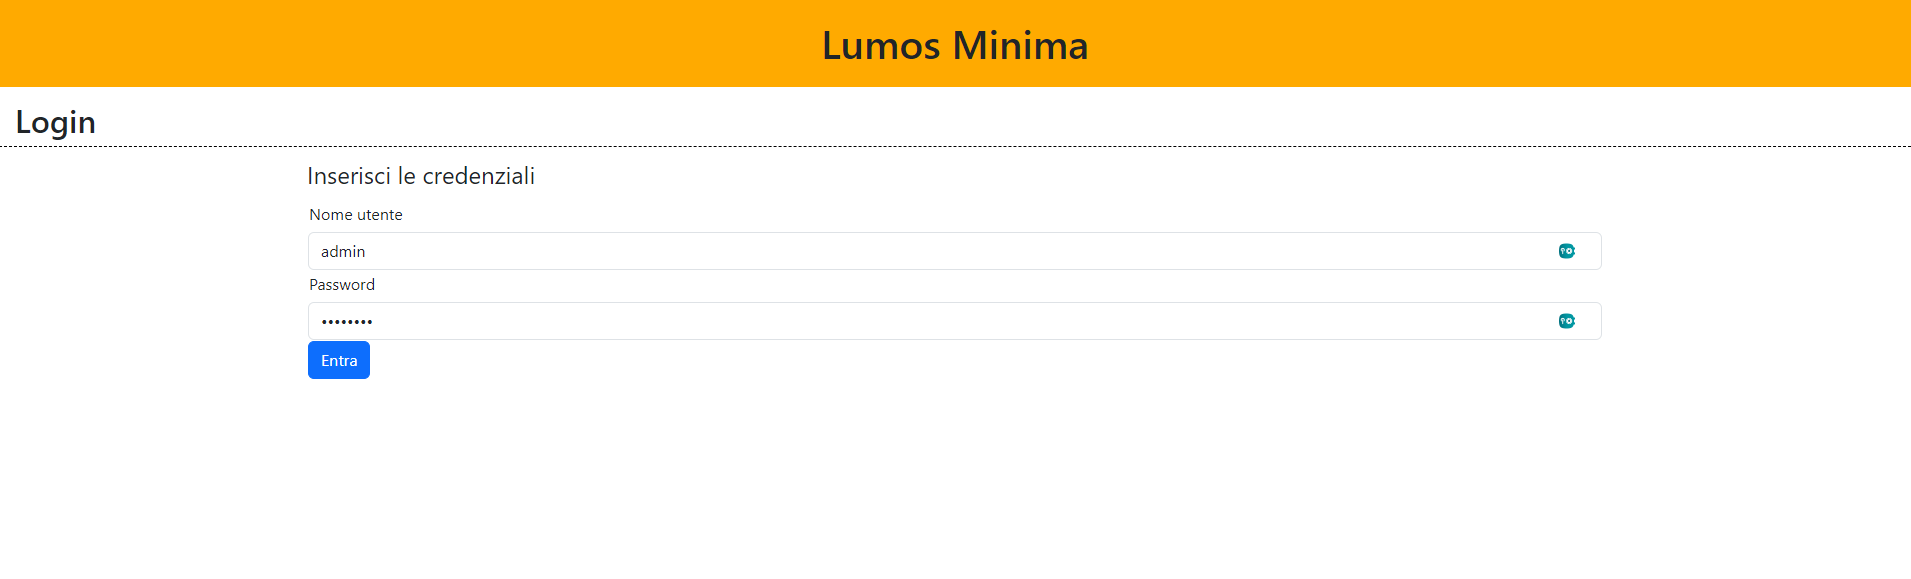
\includegraphics[width=\textwidth]{login}
\caption{Pagina di login}
\end{figure}

\subsection{Logout}
La funzionalità di logout permette di terminare la sessione generata da un precedente login non ancora scaduto. Il pulsante per il logout è posizionato nella dashboard nell'angolo in alto a destra.
% Immagine del pulsante di logout
\begin{figure}[H]
\centering

\includegraphics[width=\textwidth]{EsempioBreadcrumbConEsci}
\caption{Esempio di barra di breadcrumb con pulsante di logout}
\end{figure}

\newpage
\section{Aree Illuminate}
\subsection{Informazioni Preliminari}
Le aree illuminate sono la componente di base dell'applicazione. Esse al loro interno possono contenere molteplici lampioni e sensori che interagiscono in modo diverso coerentemente alla loro configurazione.
\subsection{Lista Aree Illuminate}
Entrando nella dashboard dopo il login, verrà presentata la lista delle aree illuminate che sono state inserite a sistema. Ogni area presenta come informazione il proprio ID (generato automaticamente), il nome assegnato, la descrizione, la latitudine e la longitudine. Al fianco di queste informazioni è presentato il pulsante per la visualizzazione delle informazioni relative a quella data area.\\
\begin{figure}[H]
\centering
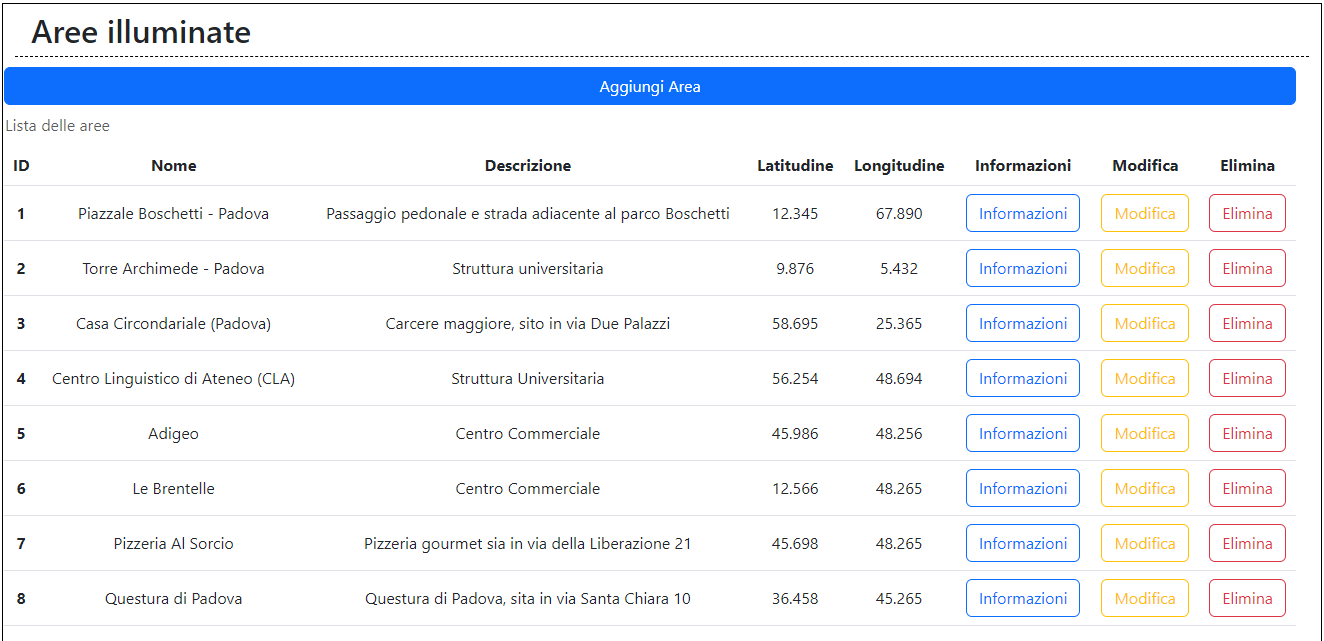
\includegraphics[width=\textwidth]{ListaAree}
\caption{Esempio di lista delle aree}
\end{figure}
Il pulsante \textit{informazioni} permette di caricare tutte le informazioni dell'area illuminata, permettendo inoltre di visualizzare i lampioni e i sensori ad essa collegati.\\
\begin{figure}[H]
\centering
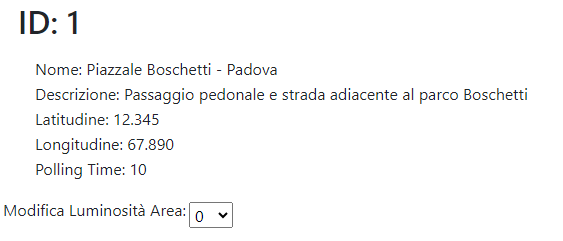
\includegraphics[width=0.5\textwidth]{InfoArea}
\caption{Esempio di informazioni di una singola area}
\end{figure}

\newpage
\section{Lampioni}
\subsection{Informazioni Preliminari}
I lampioni rappresentano la componente illuminante dell'area. Essi possono interagire in due modi diversi in base alla modalità che viene impostata:
\begin{itemize}
    \item Manuale (Pull): il lampione non si accende subito qualora il sensore rilevasse un movimento, ma utilizza il token generato dal sensore e depositato nel database e verifica ciclicamente se esiste un token valido da utilizzare;
    \item Automatico (Push): il lampione riceve un segnale di accensione istantaneo qualora il sensore rilevasse un movimento.
\end{itemize}
Inoltre, si può decidere se un lampione è recettivo rispetto ai segnali oppure no. Qualora un lampione fosse attivo (ON), allora sarà responsivo ai segnali, mentre qualora fosse disattivo (OFF) la sua gestione sarà di competenza dell'operatore umano.
\subsection{Lista Lampioni per Area}
Aprendo le informazioni di una singola area, al di sotto delle informazioni della stessa si troverà la lista dei lampioni collegati all'area selezionata.\\
Per ogni lampione, sono mostrate nella lista: l'ID (generato automaticamente), lo stato, l'intensità luminosa attuale e il nome del lampione. Al fianco di queste informazioni è presentato il pulsante per la visualizzazione delle informazioni relative a quel dato lampione.\\
\begin{figure}[H]
\centering
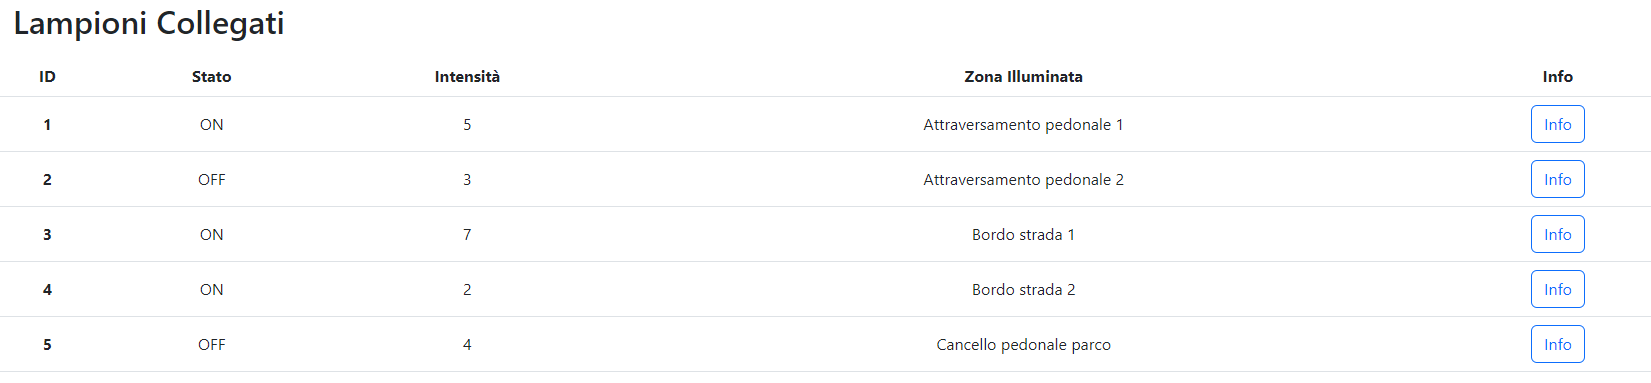
\includegraphics[width=\textwidth]{ListaLampioni}
\caption{Esempio di lista dei lampioni}
\end{figure}
Il pulsante \textit{informazioni} permette di caricare tutte le informazioni del lampione.\\
\begin{figure}[H]
\centering
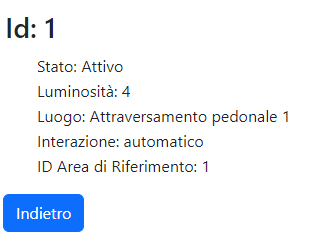
\includegraphics[width=0.5\textwidth]{InfoLampione}
\caption{Esempio di informazioni di un singolo lampione}
\end{figure}

\newpage
\section{Sensori}
\subsection{Informazioni Preliminari}
Il sensore è la componente dell'area che ha lo scopo di rilevare e di conseguenza segnalare i movimenti di cose, persone e animali nel suo raggio d'azione. Tra i suoi elementi, ne spicca uno in particolare: la durata della segnalazione. Questo parametro serve a indicare per quanto tempo i lampioni impostati in modalità manuale possano visualizzare la segnalazione come valida durante la verifica ciclica.
\subsection{Lista Sensori per Area}
\begin{figure}[H]
\centering
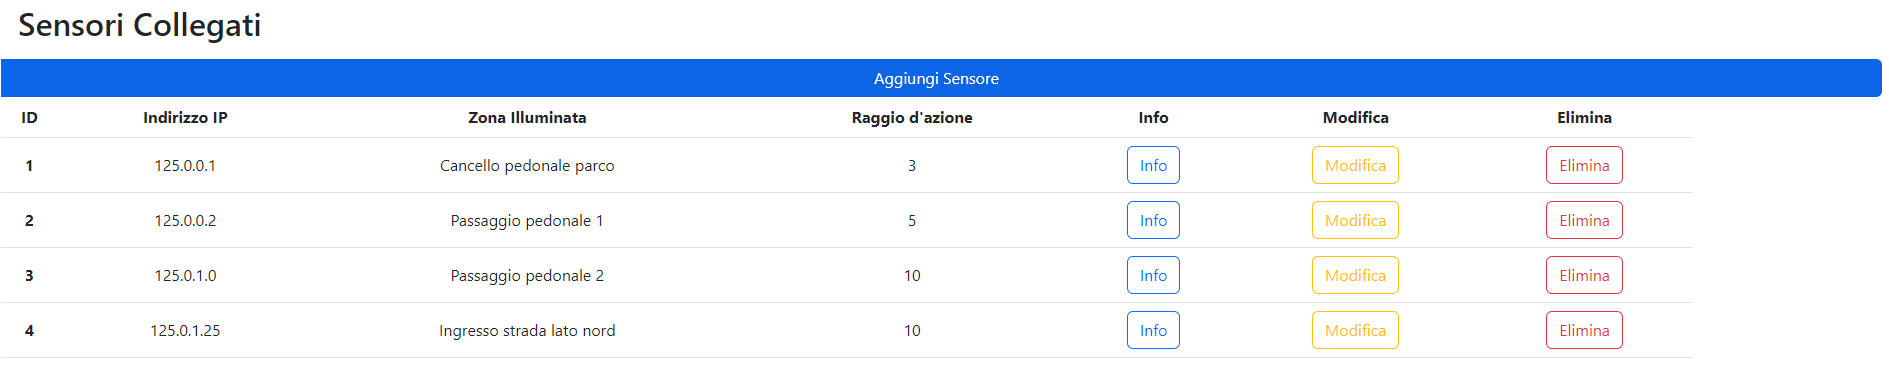
\includegraphics[width=\textwidth]{ListaSensori}
\caption{Esempio di lista dei sensori}
\end{figure}
Aprendo le informazioni di una singola area, al di sotto delle informazioni dei lampioni si troverà la lista dei sensori collegati all'area selezionata.\\
Per ogni sensore, sono mostrate nella lista: l'ID (generato automaticamente), l'indirizzo IP e il nome del sensore. Al fianco di queste informazioni è presentato il pulsante per la visualizzazione delle informazioni relative a quel dato sensore.\\
Il pulsante \textit{informazioni} permette di caricare tutte le informazioni del sensore.\\
\begin{figure}[H]
\centering
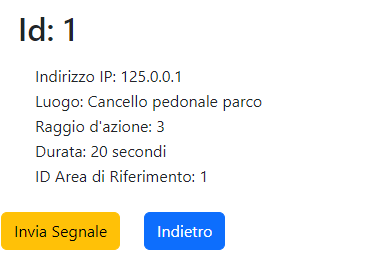
\includegraphics[width=0.5\textwidth]{InfoSensore}
\caption{Esempio di informazioni di un singolo sensore}
\end{figure}
\end{document}